\documentclass[a4paper]{article}  

\usepackage[utf8]{inputenc}
\usepackage[ngerman]{babel}	
\usepackage[babel,german=quotes]{csquotes}
%\usepackage[none]{hyphenat}
\usepackage{listings}
\usepackage{graphicx}
\usepackage{float}
\usepackage[hidelinks]{hyperref}
\usepackage{geometry}
\usepackage{wallpaper}
% may add sorting=nty later
\usepackage[backend=bibtex,defernumbers=true]{biblatex}
\usepackage{tocloft}
\parindent0pt

\geometry{
	a4paper, 
	top=25mm,
	left=40mm,
	right=25mm,
	bottom=30mm,
	headsep=10mm,
	footskip=12mm
} 

\addbibresource{../Zitate/zitate.bib}

\begin{document}

	\begin{titlepage}
		\topmargin12cm 
		\ULCornerWallPaper{1}{../Bilder/Header.jpeg}
		\begin{flushright}
			{\large Masterarbeit \\}
			\begin{Large}
				\textbf{
					Ein System zur partiellen Synchronisation \\ 
					von Wissensbasen für dezentrale soziale Netzwerke \\
				} 
			\end{Large}
			\vspace{1.0cm}
			\begin{large}	
				von Jens Grundmann \\
				\today \\
				\vspace{1.0cm}
				Hochschule für Technik und Wirtschaft Berlin \\
				Fachbereich Wirtschaftswissenschaften II \\
				Studiengang Angewandte Informatik \\
				\vspace{1.0cm}
				Erstgutachter/in Prof. Vorname Name \\
				Zweitgutachter/in Vorname Name \\	
				\vspace{0.5cm}
				\begin{center}
					
\includegraphics{../Bilder/htw_logo.jpg}
				\end{center}				
			\end{large}
		\end{flushright}	
	\end{titlepage}
	
	\ClearWallPaper	
	\newpage
	
	
	%{\LARGE \textbf{Insert later}}
	%\begin{itemize}
		%\item \hyperref[sec:sharkthemes]{Themen Shark Framework}.
	%\end{itemize} 	
	
	\newpage	
	\tableofcontents
	\newpage


	\section{Einleitung}
	
	Soziale Netzwerke erfreuen sich immer mehr Beliebtheit in den letzten Jahren. 
	Sei es Facebook oder schlicht das Forum zum Online Game, dass man gerade
	spielt. Der Mensch möchte sich austauschen. Allerdings spätestens seit den
	Enthüllungen Edward Snowdens gegen Ende Mai 2013 stellt sich hier die Frage
	der Sicherheit der persönlichen Daten. Die meisten sozialen Netzwerke basieren
	auf einer Client-Server Architektur. Dies beutetet, dass alle Daten auf einem
	entfernten Server gespeichert sind. Der Nutzer hat somit keine Kontrolle bzw.
	nur die beschränkte Kontrolle, welche der Betreiber des sozialen Netzwerkes
	anbietet, wie mit seinen Daten umgegangen wird. \\
	
	Dies ist Motivation für ein Umdenken. Anstatt die Daten an zentraler Stelle
	zu speichern verbleiben sie auf den lokalen Systemen der Benutzer. Das
	Client-Server Modell wird durch ein Peer to Peer Model ersetzt. Daten
	werden nur mit den Personen ausgetauscht, für die sie bestimmt sind.
	Hier ist eine Methode benötige, welche die Daten der lokalen Systeme
	mit einander synchronisiert. \\

	Ziel dieser Arbeit ist es eine Softwarekomponente zu entwickeln, die eine 
	partiellen Synchronisation von Wissensbasen ermöglicht. Eine Wissensbasis
	ist dabei nichts anderes als ein eine Menge an Daten, die in einer
	bestimmten Stuckatur vorliegen bzw. durch eine abstrakte Darstellung
	beschreibbar sind. Mittels dieser abstrakte Darstellung soll die 
	Implementierung von Chats, Foren bis hin zu Source Code Management Systemen
	auf einer Peer to Peer Basis vereinfacht werden.
	Als Grundlage dient hierzu das Shark Framework \cite{SharkFW} von Prof.
	Dr.	Thomas Schwotzer und die darin enthalte SyncKB Klassensammlung. Diese
	ermöglicht bereits eine Synchronisation aller Daten in einer Wissensbasis.
	Diese soll nun dahingehen ausgebaut werden, dass Teile der Wissensbasis
	beschrieben werden können und nur diese beschrieben Teile synchronisiert 
	werden. \\
	
	Zuerst muss mit eine Möglichkeit gefunden werden, wie ein Teilbereich der
	Wissensbasis beschrieben werden kann. Diese müssen dann	zwischen den 
	einzelnen Peers kommunizierbar und auf den lokalen Systemen der Peers
	persistierbar sein. Die durch diese Beschreibungen extrahierten Daten
	werden synchronisiert, wobei der Peer auf diese Aktion regieren kann um
	sie beispielsweise in einer grafischen Oberfläche auszugeben. Hierbei
	ist darauf zu achten, dass die Beschreibung so abstrakt gewählt wird, dass 
	sie	auf möglichst viele Fälle, wie die erwähnte Möglichkeit der 
	Implementierung von Chats oder Foren, anwendbar ist. \\à
	Als Beweis der Funktionalität der Softwarekomponente wird schließlich
	eine Chat mit grafisch Oberfläche geschrieben, in dem einzelne Peers sich
	miteinander	unterhalten können.\\
	
	Die Arbeit wird zuerst die Grundlagen, wie das Shark Framework \cite{SharkFW},
	auf denen die Implementierung beruht, erläutern. Danach wird das Konzept
	der Softwarekomponente erstellt. Es werden verschieden Möglichkeit
	diskutiert, um die im letzten Absatz beschriebenen Anforderungen umzusetzen.
	Im Anschluss wird die eigentliche Implementierung vorgestellt und auf
	diese eingegangen. Nachfolgend werden die Tests und Methoden nur
	Qualitätssicherung gezeigt und erklärt. Zuletzt wird ein Fazit gezogen
	sowie ein Ausblick auf mögliche Verbesserungen oder Erweiterungen.

	\newpage
	
	\section{Grundlagen}
	
	Das folgende Kapitel widmet sich den Grundlagen, auf denen die Arbeit
	beruht. Neben den Funktionale und nicht funktionale Anforderungen
	der zu entwickelnden Softwarekomponente werden Framesworks und Modelle
	besprochen, die zur Entwicklung der Komponente und Umsetzung der Anfordern
	genutzt werden können. 
	
	\subsection{Funktionale und nicht funktionale Anforderungen}
	\label{sec:requirements}
	
	Im Folgendem werden die funktionalen und nicht funktionale
	Anforderungen besprochen. Diese	beschreiben welche Features die
	Softwarekomponente bereitstellen soll, sowie wichtige Aspekte der
	Qualitätssicherung.
	
	\paragraph{Funktionale Anforderungen}
	\begin{itemize}
		\item \textbf{Beschreibbarkeit:} Es ist möglich einen Raum von
		Daten zu beschreiben und diesen von einem anderen Raum
		von Daten abzugrenzen. 
		\item \textbf{Beziehungen:} Es ist möglich Beziehungen zwischen
		Räumen zu definieren. So soll beispielsweise der Raum Java-Chat ein 
		Kind des Programmiersprachen-Chat Raumes sein können.
		\item \textbf{Persistenz:} Es soll möglich sein die Beschreibung der
		Räume von Daten persistent zu speichern. Die gespeicherten Räume
		bleiben somit erhalten und und können zu späterem Zeitpunkt neu
		geladen werden.
		\item \textbf{Synchronisation:} Es ist möglich die Räume von Daten 
		und ihre Abhängigkeiten mit Peers in einem Peer to Peer Netzwerk 
		zu synchronisieren. Ziel ist es, dass die Räume nach der 
		Synchronisation identisch von Aufbau und Inhalt sind.
		\item \textbf{Änderbarkeit:} Es muss möglich sein eine Beschreibung
		eines Raumes zu ändern inklusive ihrer Abhängigkeiten. Der Raum
		selbst soll dabei bestehe bleiben und ohne weiteren Aufwand auffindbar 
		wie	zuvor. Das heißt, er muss genauso aus der seiner persistenten Form 
		geladen werde können wie zuvor.
		\item \textbf{Änderung kommunizieren:} Änderungen müssen
		kommuniziert werden können, sodass sich andere Peers synchronisieren.
	\end{itemize} 	
	
	\paragraph{Nicht funktionale Anforderungen}
	\begin{itemize}
		\item \textbf{Build-Management:} Die Softwarekomponente ist mittels
		eines zu bestimmenden Build Tools so eingerichtet, dass das Aufsetzen 
		der	Entwicklungsumgebung für andere Entwickler schnell und einfach
		zu erledigen ist. Mögliche Synergien des gewählten Tools mit anderen
		Systemen zur Softwareentwicklung und Qualitätssicherung, zum Beispiel  
		Jenkins \cite{Jenkins}, sind wünschenswert.
		\item \textbf{Testbarkeit:} Die zu Softwarekomponente
		ist modular so aufgebaut, dass sie durch Modultest testbar ist.
		\item \textbf{Modultest:} Es existieren bereit eine Reihe von
		Modultest, welche die grundlegende Funktionalität der 
		Softwarekomponente sicherstellen.
		\item \textbf{Wartbarkeit:} Der Code der Software soll wartbar sein.
		Dies bedeutet der muss verständlich geschrieben sein und Fehler müsse
		möglichst einfach aufspürbar sein.
	\end{itemize} 
	
	\subsection{Shark Framework}
	
	In diesem Unterkapitel wird auf die grundlegenden Features des Shark
	Framework \cite{SharkFW} eingegangen, die für die Arbeit benötigt werden. 	
	Das gesamte	Framework wird nicht erklärt. Weiterführende Informationen sind
	im Developer Guide \cite{SharkManual} zu finden.
	
	\subsubsection{Context Space} 
	\label{sec:CS}
	
	Die wichtigste Grundlage ist die Context Space, der hier vereinfacht Kontext
	genannt werden soll. Hierbei handelt es sich um eine Datenstruktur.
	\autoref{fig:CSModel} zeigt ein vereinfachtes Modell dieser Struktur.
	
	\begin{figure}[H] 
		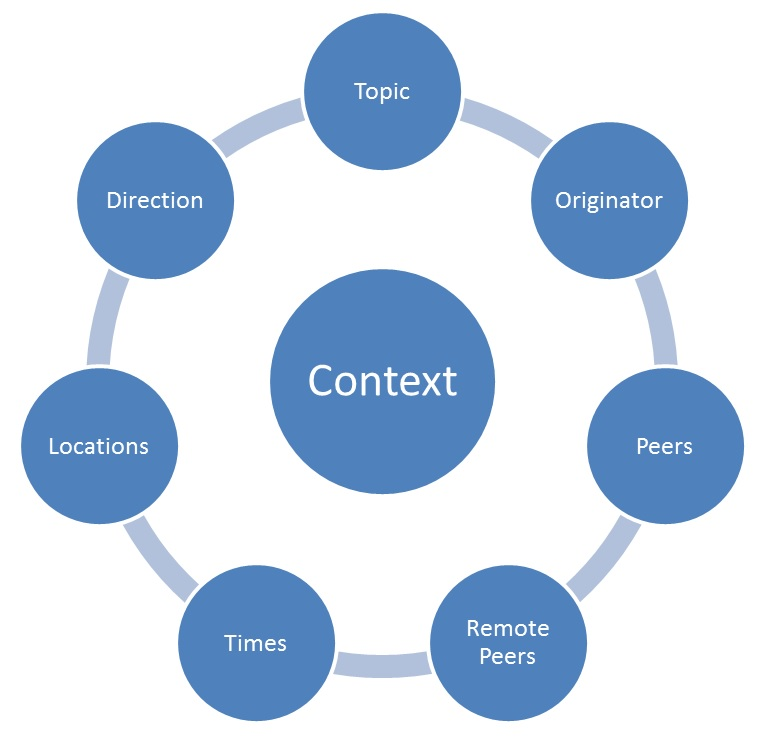
\includegraphics[width=\linewidth]{../Bilder/contextspace.jpg}
		\caption{Shark Context Space Modell}
		\label{fig:CSModel}
	\end{figure}
	
	Die einzelnen Elemente haben dabei folgende Bedeutung:
	\begin{itemize}
		\item \textbf{Topic:} Dies ist das Thema eines Kontextes. Es ist ist eine
		Beschreibung was der Kontext bedeutet.
		\item \textbf{Orginator:} Der Autor der des beschrieben Kontextes. Die
		kann entweder der Ersteller der sein oder Autor der beiliegen
		Informationen. Bei einem wissenschaftlichen Artikel wäre dies der Autor
		des Titels.
		\item \textbf{Peers:} Peers kann unterschiedlich interpretiert werden.
		Zum einen kann es der Ersteller des Kontextes sein, der sich vom Autor
		der beiliegenden Informationen unterschieden kann. Zum anderen kann es
		der Besitzer des eines Kontextes sein, wobei Besitzer hier je nach 
		beiliegendem Fall anders interpretiert werden kann. Im Allgemeinen
		kommt die Interpretation dieser auf den vorliegenden Fall an.
		\item \textbf{Remote Peers:} Dies sind die Peers an welche der Kontext
		gesendet werden soll.
		\item \textbf{Times:} Eine Zeitinformation die je nach vorliegendem Fall
		anders Interpretiert weiden kann. Diese Dimension biete die Möglichkeit
		ein Zeitintervall anzugeben.
		\item \textbf{Locations:} Gibt einen Ort an. Diese Information kann je
		nach vorliegendem Fall anders interpretiert werden.
		\item \textbf{Direction:} Die Richtung der Kommunikation des Kontextes.
		Es ist möglich nur Informationen über einen Kontext zu empfangen, sie nur
		zu senden, zu lesen und senden und keine der genannten Aktionen
		durchzuführen.
	\end{itemize} 	
	
	Zu beachte ist, dass wenn von einem Kontext gesprochen wird, dann handelt es
	sich hierbei um eine Beschreibung einer Menge von Kontextpunkten. Diese
	Punkte haben den gleichen Aufbau wie in \autoref{fig:CSModel} gezeigt. Der 
	wesentliche Unterschied ist, dass ein Kontext eine Vielzahl von Inhalten,
	ausgenommen der Direction, besitzen kann. Wehrendessen besitzt der
	Kontextpunkt nur je genau einen Inhalt. Beispielhaft beschriebt der
	Kontextpunkt nur das Thema Java, während der Kontext Java und C++ beinhaltet.
	Die Dimensionen selbst werde als Kontextkoordinaten bezeichnet. Der 
	Kontextpunkt vereint Koordinaten und Informationen. Der Kontext wiederum
	ist eine Möglichkeit eine menge an Kontextpunkten aus einer zugrundeliegenden
	Wissensbasis zu extrahieren.
	
	\subsubsection{Knowledge Base} 
	Die Knowledge Base, zu deutsch Wissensbasis, ist Eine Sammlung von Wissen.
	Wissen ist dabei eine Menge an Informationen, die anhand von
	Kontextkoordinaten beschrieben sind. Die Vereinigung von Kontextkoordinaten
	und Informationen bildeten einen Kontextpunkt.\\
	
	Die Wissensbasis bietet die Möglichkeit Peers und Themen zu speichern, sowie
	die Themen in einer Taxonom einzuordnen. Der für die zu entwickelnde
	Softwarekomponente wichtige Punkt ist aber die Möglichkeit genannte
	Kontextpunkt in ihr zu speichern und anhand eines Kontextes zu extrahieren.
	Die Wissensbasis selbst kann hierbei ähnlich einer Datenbank angesehen werden.
	Ziel ist es Teilbereiche, sprich eine bestimmte Menge an Daten dieser, mit
	anderen Wissensbasen zu synchronisieren. Zu diesem Zweck gebt es bereits eine
	Implementierung, SyncKB genannt, auf der aufgebaut wird. \\
	
	Zusätzlich zu den genannten Eigenschaften gibt es die Properties an der
	Wissensbasis zu speichern. Dies sind Name-Wert-Paare, wobei sowohl Name 
	als auch Wert eine Zeichenkette ist.
	
	\subsubsection{Knowledge Port} 
	Das wichtigste Objekt zur Kommunikation im Peer to Peer Netzwerk vom Shark
	Framework ist der KnowledgePort. Hierbei handelt es um eine abstrakte Klasse,
	welche die Implementierung von \emph{doExpose(SharkCS interest, KEPConnection
	kepConnection)} und \emph{doInsert(Knowledge knowledge, KEPConnection
	kepConnection)} erfordert. \\
	
	Die doExpose-Methode erhält ein Interesse in der Form eines SharkCS. Wenn
	ein Interesse versandt wurde, so wird sie als Erstes aufgerufen. Ihre 
	generelle Aufgabe ist zu ermitteln, ob das Interesse für, das erhalten wurde, 
	für den KnowledgePort von Relevanz ist. \\
	
	Die doInsert-Methode hingegen erhält ein Knowledge Objekt, welches echte
	Daten enthält. Es wird in der Regel gegen Ende der Kommunikation auf gerufen
	und soll die Daten in die Wissensbasis einfügen. \\
	
	Beide Methoden erhalten ein KEPConnection Objekt mit dem sie Informationen 
	über den Sender erhalten können. Des Weiteren kann mithilfe dieses 
	Objektes Daten an die doExpose und doInsert-Methode anderer Peer gesendet
	werden. Dies erlaubt einen mehrfachen Datentausch. Ein Beispiel hierzu ist
	der Synchronisationsprozess der SychKB, der im Nächten Abschnitt beschrieben 
	wird und in \autoref{fig:SyncSeq} skizziert ist. \\
	
	Zu beachten ist, dass die Aussagen hier dem Standardfall entsprechen, wonach
	der Knowledge Port entworfen wurde. Die tatsächliche Implementierung und
	damit der Umgang mit dem SharkCS Objekt und dem Knowledge kann von jedem
	Entwickler selbst bestimmt werden.Einzig vorgeschrieben ist, dass zuerst
	ein Interesse versandt wird und Daten in der Form eines Knowledge Objektes
	gesendet werden.
	
	\subsubsection{SyncKB}
	\label{sec:SyncKB}
	
	Leider gibt es, abgesehen der Javadoc Dokumentation, keine genaue
	Beschreibung der Funktionsweise der SyncKB. Daher soll hier auf die
	generelle Funktionsweise dieser eingegangen werden. Weitere Informationen
	können den Quellcode selbst entnommen werden, der im Github vom SharkFW
	zu finden ist. \cite{SyncKB} \\
	
	Die SyncKB enthält den Hauptteil ihrer Logik im SyncKP. Die eigentliche
	Synchronisation findet während des Kommunikationsprozesses statt und ist
	keine Eigenschaft der Wissensbasis selbst. Die einzelnen Elemente der SyncKB
	basiert hauptsächlich auf dem Entwurfsmuster Wrapper. So wurden den einzelnen
	Element zwei zusätzliche Informationen mitgeben: 
	
	\begin{itemize}
		\item \textbf{Version:} Die Aktuelle Version des Elements. Ein neu 
		erstelltes Element startet bei 1 und bei jeder Änderung wird die
		Version um eins erhöht.
		\item \textbf{Zeitstempel:} Ein Zeitstempel der angibt, wann die letzte
		Änderung an dem Element vorgenommen wurde.
	\end{itemize} 
	
	Wie erwähnt befindet sich der Großteil der Logik im SyncKP.
	\autoref{fig:SyncSeq} zeigt die ablaufende Kommunikation zwischen zwei
	Peers, die hier vereinfacht Alice und Bob genannt werden sollen.	
	
	\begin{figure}[H] 
		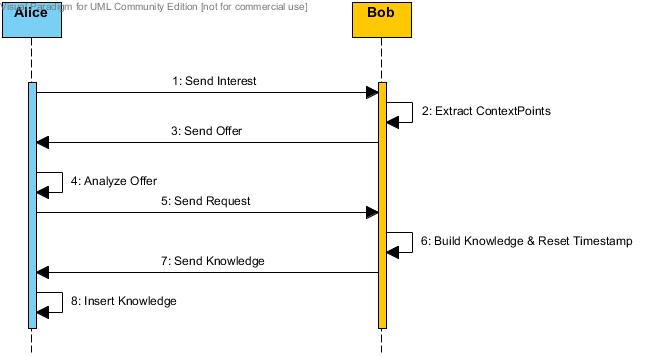
\includegraphics[width=\linewidth]{../Bilder/sync_seq.jpg}
		\caption{Kommunikation der SyncKB}
		\label{fig:SyncSeq}
	\end{figure}
	
	\begin{enumerate}
		\item \textbf{Interesse senden:} Der Prozess beginnt damit, dass Alice
		ihr Interesse zur Synchronisation verkündet. Das hierbei gesendete
		Interesse ist ein künstliches Interesse. Es wird vom SyncKP intern
		verwendet und dient lediglich als Datenhalter für diesen.
		\item \textbf{Kontextpunkte extrahieren:} Nachdem das Interesse an der
		Synchronisation Bob erreicht hat stellt dieser ein Angebot für Alice
		zusammen. Im linken Teil von \autoref{fig:SyncFlow} ist der
		Algorithmus dazu skizziert. Hierbei wird ausgenutzt, dass an jedem
		SyncContextPoint ein Zeitstempel der letzten Änderung gespeichert ist.
		Dieser wird mit dem Zeitpunkt des letzten Treffens mit dem Peer,
		das die Synchronisation anfordert, verglichen. Dazu ist an der
		Wissensbasis, per Property, eine Liste von Name-Wert-Paare gespeichert, 
		welche den Zeitpunkt des letzte Treffen mit einem Peer enthält.
		Genauer ist ein Peer jeweils einem Zeitstempel zugeordnet. Alle
		Kontextpunkte, deren letzte Änderung neuer ist als das letzte Treffe mit
		einem spezifischen Peer, hier Alice, werden angeboten.
		\item \textbf{Angebot senden:} Die extrahierten Kontextpunkte werden per
		Property am künstlichen Interesse Alice als Angebot zugewendet. Zu beachten
		ist dabei, dass nur die Daten eines Kontextpunktes versendet werden.
		Eventuelle Informationen, die diesem zugeordnet sind, werden nicht
		versandt.
		\item \textbf{Angebot analysieren:} Alice analysiert das Angebot, dass
		sie von Bob erhalten hat. Der Algorithmus ist ähnlich dem späteren Einfügen
		von der Kontextpunkte und im rechten Teil von \autoref{fig:SyncFlow}
		skizziert. Alice wird alle Kontextpunkte von Bob anfragen, die sie
		nicht besitzt oder die bei Bob eine höhere Versionsnummer haben als
		bei ihr selbst.
		\item \textbf{Anfrage senden:} Die anzufragenden Kontextpunkte werden
		abermals am künstlichen Interesse per Property gespeichert und Bob
		zugesandt.  
		\item \textbf{Wissen bauen und Zeitstempel zurücksetzen:} Die angefragten
		Kontextpunkte werden nun aus Bobs Wissensbasis extrahiert und in einem
		Knowledge Objekt gespeichert. Zusätzlich werden	alle Themen und Peers,
		anhand der beim Erstellen des SyncKP übergebenen FragmentationParameter,
		dem Knowledge Objekt übergeben.
		\item \textbf{Wissen senden:} Das Knowledge Objekt wird nun an Alice
		gesendet.
		\item \textbf{Wissen in Wissensbasis einfügen:} Alice überprüft das
		die Kontextpunkte anschließend noch einmal anhand das im rechten Teil von
		\autoref{fig:SyncFlow} skizzierten Algorithmus und fügt diese dann in
		ihre Wissensbasis ein.
	\end{enumerate} 	
	
	\begin{figure}[H] 
		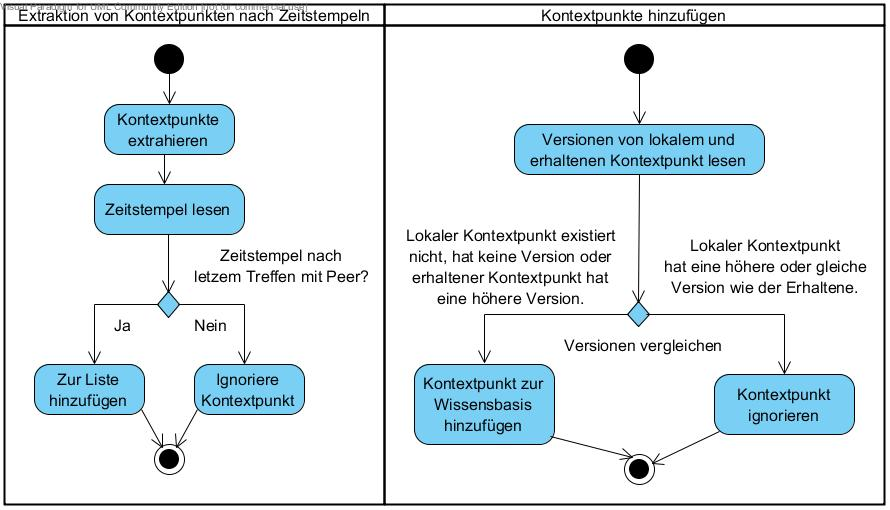
\includegraphics[width=\linewidth]{../Bilder/sync_flow.jpg}
		\caption{Algorithmus zum Extrahieren und Einfügen von Wissen der SyncKB}
		\label{fig:SyncFlow}
	\end{figure}
	
	Das System von Angebot und Anfrage wird verwendet, um das Datenvolumen während
	der Kommunikation möglichst gering zu halten. Wie erwähnt enthalten Angebot
	und Anfrage nur die nötigen Informationen zu den Kontextpunkten, wie
	Koordinaten, Zeitstempel und Version, und zusätzlich mit dem Punkt verknüpften
	Informationen. Erst gegen Ende des Synchronisationsalgorithmus wird ein 
	Objekt mit den vollständiges Daten erstellt und versandt.
	
	\subsection{Datenstrukturen zur Darstellung von Beziehungen}
	\label{sec:datastruct}
	
	Wie in Abschnitt \ref{sec:requirements} beschrieben soll es möglich sein
	Abhängigkeiten zwischen Räumen aufzustellen. Diese Abhängigkeiten stellen
	eine Beziehung zwischen Daten da. Daher werden in diesem Abschnitt 
	Datenstrukturen besprochen, die eine solche Beziehung darstellen können.
	Dabei wird darauf eingegangen, wie sie die Daten und Beziehungen untereinander
	dargestellt sind. Weitergehende Erklärungen, wie mögliche Operationen, werden
	nur durch Links zu entsprechender Literatur gegeben.
	
	\subsubsection{Verkette Listen}
	
	Verkette Listen (beschrieben in \cite{FundData}, Kapitel 4) sind Listen,
	wo jedes Element Referenzen auf weitere Mitglieder der Liste einhält.
	Hier sollen die Einfach-Verketteten-Listen und die Zweifach-Verketten-Listen
	betrachten werden.
	
	\paragraph{Einfach-Verkettete-Listen}\mbox{} \\
	
	Einfach-Verkettete-Listen besitzen eine Referenz auf ihren Nachfolger.
	Die Beziehung der einzelnen Elemente ist hierbei, dass jedes Element
	seinen Nachfolger kennt, nicht aber seinen Vorgänger. Die Beziehungen
	können also nur vorwärts verfolgt werden, das heißt von einem Element
	Zum nachfolgenden, nicht aber von einem Element zum Vorherigen.
	\autoref{fig:single_linked_list} skizziert dieses und zeigt mögliche
	Operation an einer verketteten Liste. weitere Informationen können
	der Erklärungen unter \cite{SLList} entnommen werden.
	
	\begin{figure}[H] 
		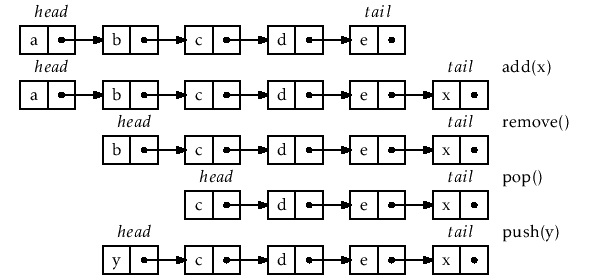
\includegraphics[width=\linewidth]{../Bilder/single_linked_list.jpg}
		\caption
		{
			Aufbau und Operation einer einfach verketteten Liste.
			Quelle: \cite{SLList}
		}
		\label{fig:single_linked_list}
	\end{figure}	
	
	\paragraph{Zweifach-Verkette-Listen}\mbox{} \\
	
	Zweifach-Verkette-Listen besitzen, gegenüber Einfach-Verkettete-Listen,
	eine Referenz auf Vorgänger und Nachfolger. Die Beziehung der einzelnen
	Elemente ist also, dass jedes Element seinen Vorgänger und Nachfolger
	kennt. Somit kann die Liste vorwärts, von Element zum nachfolgenden
	Element, als auch rückwärts, vom Element zum vorhergehenden Element
	verfolgt werden. \autoref{fig:double_linked_list} skizziert dieses.
	Weitere Informationen können den Erklärungen unter \cite{DLList} entnommen
	werden.
	
	\begin{figure}[H] 
		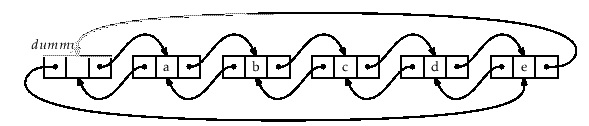
\includegraphics[width=\linewidth]{../Bilder/double_linked_list.jpg}
		\caption
		{
			Aufbau einer zweifach verketteten Liste.
			Quelle: \cite{DLList}
		}
		\label{fig:double_linked_list}
	\end{figure}	
	
	\subsubsection{Bäume}
		
	Bäume (\cite{FundData}, Kapitel 4) bestehen aus einem Wurzelknoten
	und weiteren Knoten, die von diesem ausgehen. Hierbei besteht eine Vater-Kind
	Beziehung zwischen diesen. Die Wurzel besondere Eigenschaft der ist, dass
	sie keinen Vater besitzt. Knoten, die keine Kinder besitzen, werden Blätter
	genannt. Ein Element kann hier also beliebig vielen Unterelementen, seinen
	Kindern, in Beziehung stehen. Hingegen kann ein Element von nur einem anderen
	Element abstammen. \autoref{fig:tree} skizziert ein Beispiel
	dieser Datenstruktur.
	
	\begin{figure}[H] 
		\centerline{
			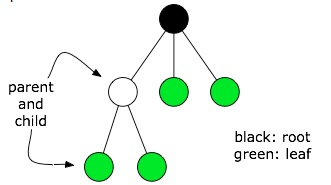
\includegraphics{../Bilder/tree.jpg}
		}
		\caption
		{
			Aufbau eines Baums.
			Quelle: \cite{Trees}
		}
		\label{fig:tree}
	\end{figure}
	
	\subsubsection{Graphen}
	
	Graphen (siehe \cite{FundData}, Kapitel 6) bilden ein Netz von Daten. Dabei
	kann von jedem Element eine Beziehung zu einem anderen ausgehen. Gegenüber
	Bäumen besitzen sie keine Wurzel, der den Anfang darstellt. Zudem sind die
	Beziehungen nicht fest gelegt. Ein Element besitzt eine Vielzahl an
	Beziehungen. Gerichtet Graphen geben dieser Beziehung eine Richtung.
	Somit kann allerdings nur angeben werden von welchem Element man zu welchen
	gelangt und gegebenenfalls nicht mehr zurück. Dies ist ähnlicher dem 
	Nachfolger Link in einer verketteten Liste und stellt nicht,
	wie beim Baum, eine Vater Kind Beziehung da. Des Weiteren besteht die
	Möglichkeit in gewichteten Graphen Metadaten, wie die Kosten für einen
	Übergang von Element A zu Element B, den Richtungen mitzugeben. Dennoch bleibt
	die Art wie zwei Elemente im Detail zueinander in Beziehung stehen	
	umbeschrieben. \autoref{fig:graph} skizziert das Modell eines gerichteten
	Graphen. Die Peile stellen dabei die Übergänge zwischen den Elementen da.
	Weitere Erklärungen könne unter \cite{Graph} gefunden werden. 

	\begin{figure}[H] 
		\centerline{
			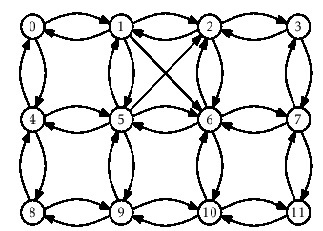
\includegraphics{../Bilder/graph.jpg}
		}
		\caption{Aufbau eines Graphen. Quelle: \cite{Graph}}
		\label{fig:graph}
	\end{figure}
	
	\subsubsection{Entity Relationship Modell}
	
	Das Entity Relationship Modell, beschrieben in \cite{EntRel}, ist weniger
	ein Datenstruktur als ein Modell zur Beschreibung von Zusammenhängen zwischen
	Daten bekannt aus relationalen Datenbanksysteme. Damit beschriebt es aber
	auch eine Beziehung und kann somit als Grundlage herangezogen werden. Die
	Beziehungen basieren darauf, dass jede Element einen eindeutige 
	Primärschlüssel besitzt. Datensätze, die mit anderen Datensätze in Beziehung 
	stehen, besitzen einen Fremdschlüssel, welcher identisch zum Primärschlüssel
	des Datensatzes ist, mit dem sie in Beziehung stehen. \autoref{fig:ent_rel}
	zeigt eine vereinfachte Skizze dieser Beziehung auf. anders als die Abbildung
	erscheinen lässt sind diese Schlüssel nicht an einen Datentypen gebunden. Auch
	kann ein Schlüssel mehre Daten eines Datensatzes umfassen. Die Trennung
	in Primärschlüssel und Fremdschlüssel erlaubt auch die Art der Beziehung zu
	interpretieren. Beispielsweise kann dies eine Vater-Kind-Beziehung darstellen.
	Das Modell ist aber nicht an diese Interpretation gebunden.
	
	\begin{figure}[H] 
		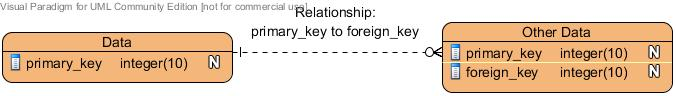
\includegraphics[width=\linewidth]{../Bilder/ent_rel.jpg}
		\caption{Vereinfachte Skizze des Entity Relationship Modell}
		\label{fig:ent_rel}
	\end{figure}	
	
	\subsection{Aufbau von Social Media Formaten}	
	\label{sec:social}
	
	In diesem Abschnitt soll der Aufbaue eine Reihe von Social Media Formaten
	beschrieben werden. Social Media Formaten sind dabei Anwendungen, die
	den Kontakt mit anderen Menschen fördern. Die Verknüpfung der einzelnen
	Informationen und Daten miteinander soll hierbei von besonderem Interesse sein,
	da sie die Abhängigkeiten aus Abschnitt \ref{sec:requirements} darstellen.
	
	\subsubsection{Chat}	
	
	Chats sind einer der einfachsten Möglichkeiten der Kommunikation. Abbildung
	\ref{fig:chat} zeigt den Aufbau eines Chat im Programm Skype.
	
	\begin{figure}[H] 
		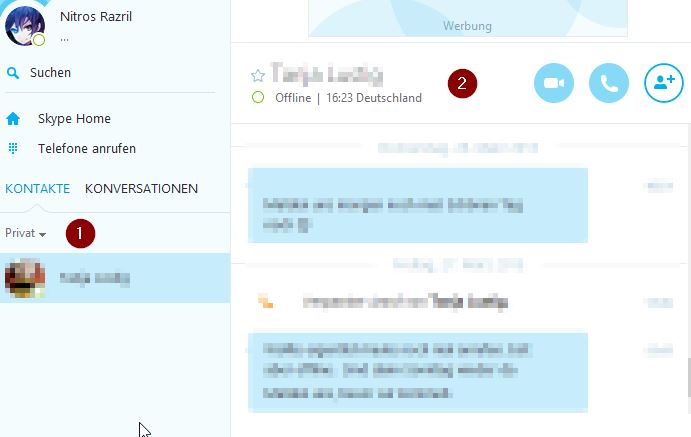
\includegraphics[width=\linewidth]{../Bilder/chat.jpg}
		\caption{Aufbau Chat in Skype. \cite{chat}}
		\label{fig:chat}
	\end{figure}		
	
	Die Aufteilung erfolgt hier in erster Ebene(1) in Gruppen. In zweiter Ebene(2)
	ist der eigentliche Chat. Ein Chat besitzt eine Vielzahl von Daten. Ein
	Eintrag einhält beispielsweise einen Zeitstempel, Text und Autor der
	Nachricht. Der Chat selbst erscheint identifizierbar durch einen nicht
	sichtbaren Identifikator, da Elemente wie Teilnehmer geändert werden können
	und der Chat trotzdem auffindbar ist. Vereinfacht kann man sagen, dass ein
	Chat eine einzelner Raum von Informationen ist, der auf eine bestimmte Art
	durch einen oder mehre Identifikatoren beschrieben sind.
	
	\subsubsection{Forum}	
	
	Ein Forum ist gegenüber den Chat meist komplexer und lässt sich in mehr
	Ebenen einteilen. Als Beispiel soll das	Burning Board der WoltLab GmbH
	herangezogen werden \cite{BB}. In den folgende Abbildungen
	\ref{fig:forumstruc001}, \ref{fig:forumstruc002} und \ref{fig:forumstruc003}
	ist der strukturelle Aufbau eines Forums zu sehen.
	
	\begin{figure}[H] 
		\centerline{
			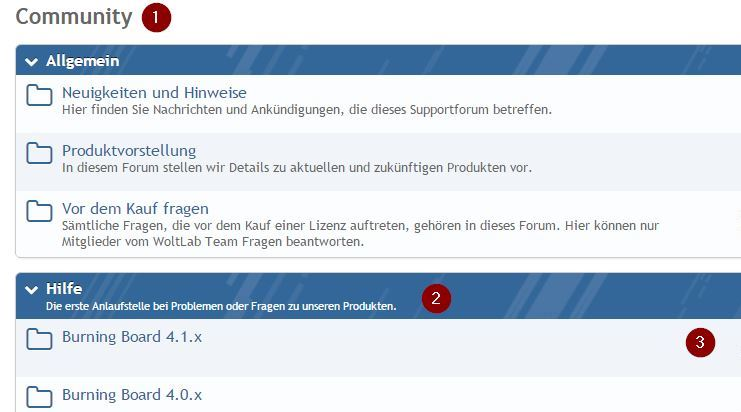
\includegraphics[scale=0.65]{../Bilder/forumstruc001.jpg}
		}
		\caption{Forumstruktur: Oberste Ebene. Quelle: \cite{BB}}
		\label{fig:forumstruc001}
	\end{figure}	
	
	\autoref{fig:forumstruc001} zeigt die oberste Ebene eines Forums. Man sieht
	eine Baumstruktur mit einer Wurzel(1). Von diesem Baum gehen Äste(2) aus
	von welchem wiederum weitere Äste(3) ausgehen können.
	
	\begin{figure}[H] 
		\centerline{
			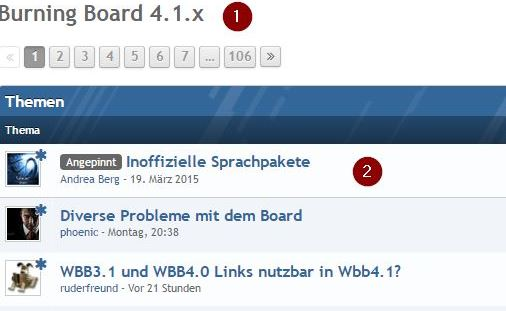
\includegraphics{../Bilder/forumstruc002.jpg}
		}
		\caption{Forumstruktur: Thread-Sammlung Ebene. Quelle: \cite{BB}}
		\label{fig:forumstruc002}
	\end{figure}	
	
	\autoref{fig:forumstruc02} zeigt die Ebene, in der die Threads mit den
	Inhalten zu finden sind. Man sieht, dass es sich hierbei um einen Konten(1)
	in der zuvor erwähnten Baumstruktur handelt. Die einzelnen Threads(2) stellen
	dabei die Blätter des Baumes da.
		
	\begin{figure}[H] 
		\centerline{
			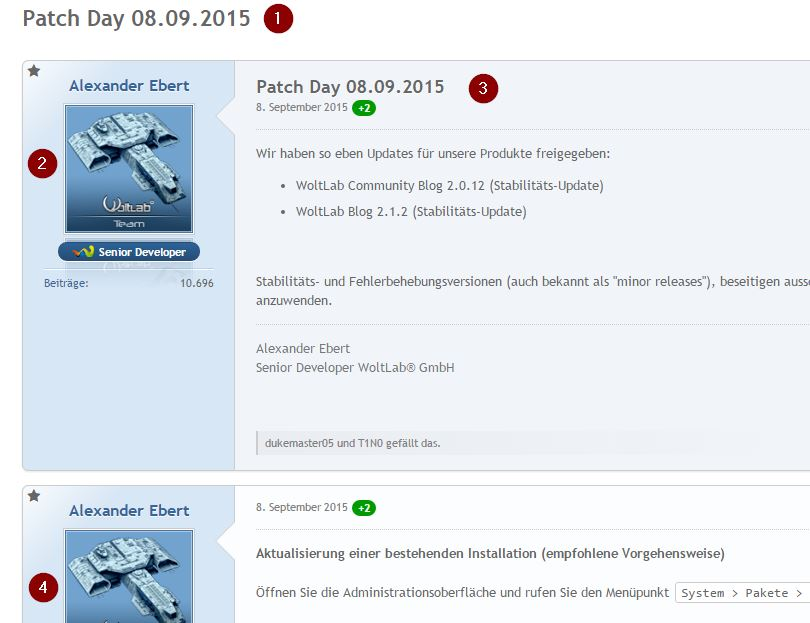
\includegraphics[scale=0.6]{../Bilder/forumstruc003.jpg}
		}
		\caption{Forumstruktur: Thread Ebene. Quelle: \cite{BB}}
		\label{fig:forumstruc003}
	\end{figure}	
	
	\autoref{fig:forumstruc003} zeigt einen Thread in einem Forum. Dieser ist
	ein Blatt(1) in der Baumstruktur. Ähnlich wie der Chat ist ein Thread ein
	Raum von Daten. Die einzelnen Einträge(3, 4) besitzen dabei genauso 
	ähnliche Daten,	wie zum Beispiel Zeitstempel, Text und Autor(2). \\
	
	Trotz des unterschiedlichen Layouts der grafischen Oberfläche besitzen
	Threads und Chat eine Vielzahl von Gemeinsamkeiten in ihrem Aufbau. Der
	größte Unterschied ist, dass Foren sich einer Baumstruktur bedienen um
	die einzelnen Raume von Daten anderen Räumen unterzuordnen. Dies kann
	als Vater-Kind-Beziehung eines Baumes gesehen werden, wobei nur die Blätter
	Daten enthalten. Andere Knoten dienen lediglich einer Ordnung der Daten und 
	der Eingruppierung dieser in einen definierten Bereich.
	
	\subsubsection{Dateisysteme und Versionsverwaltung Software}	
	
	Es mag auf den ersten Blick nicht so erscheinen, aber auch Dateien auf
	dem Dateisystem können für soziale Kontakte genutzt werden. Ein einfaches
	Beispiel hierfür ist die Existenz der die vielen Image-Hoster. Auch 
	Facebook und Instagram erlauben den Austausch von Bildern. \\
	
	In diesem Sinne kann auch Versionsverwaltung Software wie Git oder SVN als
	eine Art des sozialen Kontaktes gesehen werden. In einem Online Artikel der
	t3n \cite{articleGitHub} wird beschrieben, dass man immer mehr auf den
	webbasierter Filehosting-Dienst für Software-Entwicklungsprojekte GitHub
	\cite{gitHub} stößt, der auf Git basiert. Mit seiner Vielzahl an Projekten
	der unterschiedlichsten Programmiersprachen kann GitHub als soziale Plattform
	für Softwareentwickler gesehen werden. \\
	
	Aus diesem soll der Austausch von Teilen des Software über solche 
	Versionsverwaltung Software auch Betrachtung finden. \autoref{fig:filesytsem}
	zeigt den Allgemeinen von Dateisystem für unterschiedliche Betriebssysteme.
	
	\begin{figure}[H] 
		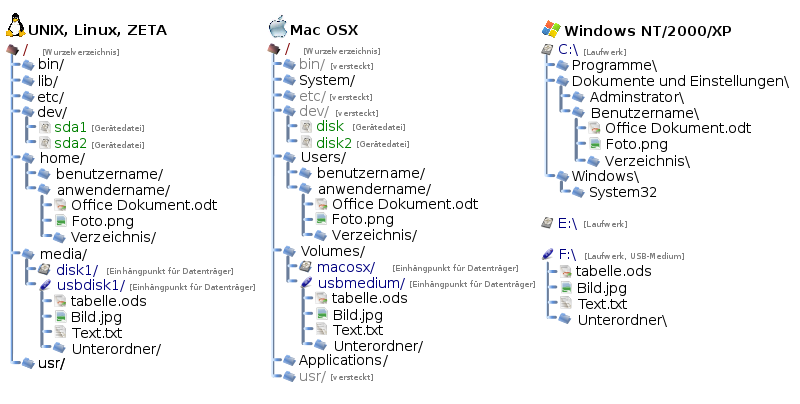
\includegraphics[width=\linewidth]{../Bilder/filesystem.png}
		\caption{
			Illustration über den Vergleich von Dateisystem-Bäumen.
			Quelle: \cite{filesytsem}
		}
		\label{fig:filesytsem}
	\end{figure}
	
	Zu sehen ist, das identisch zum Forum eine Baumstruktur die Grundlage von
	Dateisystemen ist. Ebenfalls einhalten auch hier nur die Blätter die
	die eigentlichen Daten und die anderen Knoten diene lediglich
	der Eingruppierung von Daten. Die Blätter selbst können als ein einzelnes
	Element bestehend aus Bytes angereichert mit Metadaten gesehen werden.
	Dies unterscheidet sich zum Chat oder Forum, wo ein Blatt einem beschreibbarem
	Raum von Daten bestand. 
		
	\newpage
	
	\section{Konzeption}	
	
	In diesem Abschnitt wird die Konzeption der geplanten Softwarekomponente
	besprochen. Basierend den Grundlagen des vorherigen Kapitels wird eine
	Auswahl getroffen und Techniken zur Implementieren gewählt.
	
	\subsection{Serialisierung}
	\label{sec:konz_serialisierung}
	
	Eine der Anforderungen aus dem Abschnitt \ref{sec:requirements} war Persistenz.
	Es sollte möglich sein eine Beschreibung eines Raumes zu speichern und später
	wieder abrufen zu können. Zu diesem Zweck macht es Sinn das Feature des Setzen
	von Properties an einer Wissensbasis zu nutzen. Auf diesem Weg kann je 
	Wissensbasis eine Liste von Beschreibungen gespeichert werden. Insbesondere
	kann dies als Zugrodung dieser Beschreibungen zur entsprechenden Wissensbasis
	gesehen werden. \\
	
	Dazu benötigen wir eine Technik, welche die Serialisierung eines Objektes einer
	Programmiersprache, in diesem Fall Java, in eine Zeichenkette ermöglicht. Um
	die Anforderung der Wartbarkeit zu gewährleisten soll hier ein menschlich
	lesbares Format gewählt werden, dass von den meisten Entwicklern verstanden
	wird. XML und JSON erfüllen diese Anfordern. Zum Vergleich sollen die
	Ergebnisse aus der Fallstudie \cite{XmlJson} zu rate gezogen. Diese in den
	folgenden Abbildungen dargestellt.
	
	\begin{figure}[H] 
		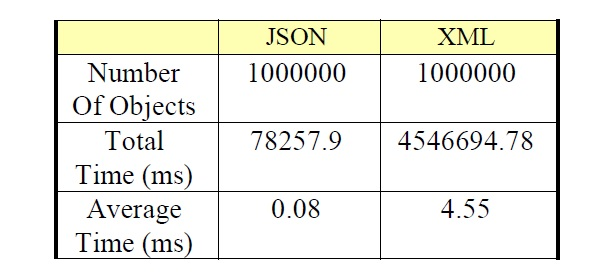
\includegraphics[width=\linewidth]{../Bilder/xml_json_time_sen1.jpg}
		\caption{Scenario 1 JSON vs. XML Timing. Quelle: \cite{XmlJson}}
		\label{fig:xml_json_time_sen1}
	\end{figure}
	
	\begin{figure}[H] 
		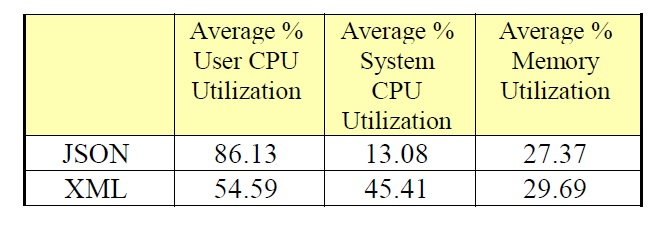
\includegraphics[width=\linewidth]{../Bilder/xml_json_mem_sen1.jpg}
		\caption{Scenario 1 JSON vs. XML CPU/Mem. Quelle: \cite{XmlJson}}
		\label{fig:xml_json_mem_sen1}
	\end{figure}
	
	\newpage
	
	Die Abbildungen \ref{fig:xml_json_time_sen1} und \ref{fig:xml_json_mem_sen1}
	zeigen den ersten Fall der Fallstudie. Hier wurde eine große Menge an Daten
	über einen Kommunikationskanal gesendet. Es ist klar ersichtlich, dass JSON
	in den Bereichen Timing und CPU/Memory eine bessere Qualität aufzeigt. Einzig
	bei der Nutzung der CPU des Nutzers zeigt XML bessere Werte auf.
	
	\begin{figure}[H] 
		\centerline{
			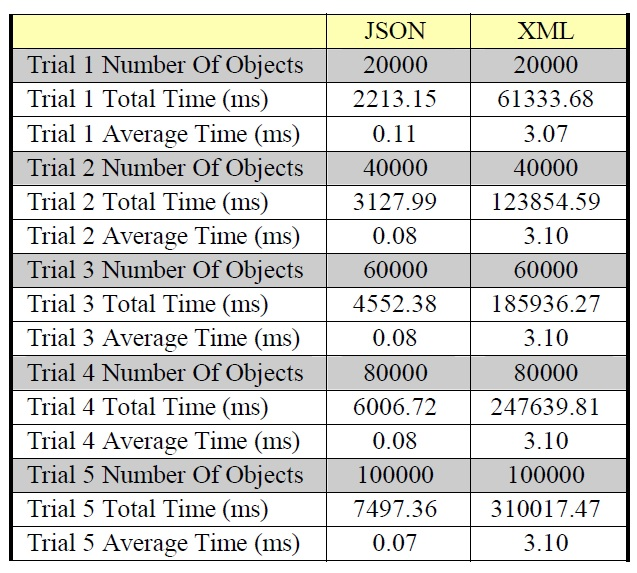
\includegraphics[scale=0.8]{../Bilder/xml_json_time_sen2.jpg}
		}
		\caption{Scenario 2 JSON Vs XML Timing. Quelle: \cite{XmlJson}}
		\label{fig:xml_json_time_sen2}
	\end{figure}
	
	\begin{figure}[H] 
		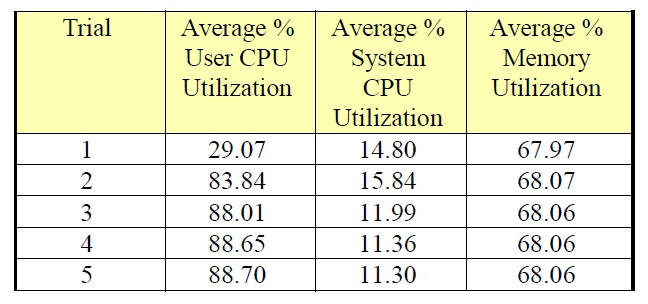
\includegraphics[width=\linewidth]{../Bilder/json_mem_sen2.jpg}
		\caption{Scenario 2 JSON CPU/Mem. Quelle: \cite{XmlJson}}
		\label{fig:json_mem_sen2}
	\end{figure}
	
	\begin{figure}[H] 
		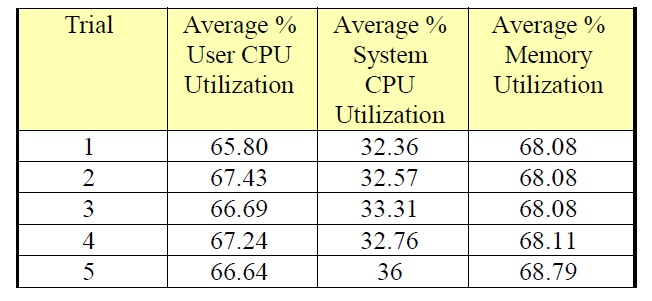
\includegraphics[width=\linewidth]{../Bilder/xml_mem_sen2.jpg}
		\caption{Scenario 2 XML CPU/Mem. Quelle: \cite{XmlJson}}
		\label{fig:xml_mem_sen2}
	\end{figure}
	
	Die Abbildungen \ref{fig:xml_json_time_sen2}, \ref{fig:json_mem_sen2}
	und \ref{fig:xml_mem_sen2} zeigen den Zweiten Fall der Fallstudie. Hier
	wurden mehrfach hintereinander kleine Datensatze überragen anstatt alle
	Datenobjekte in einer Übertragung zu senden. Auch hier zeigt sich, dass
	JSON im allgemeinen bessere Werte liefert. Nur bei der Nutzung der CPU des
	Nutzers zeigt XML, wie im ersten Fall, bessere Werte auf. \\
	 
	Mit den vorliegenden Daten würde die Wahl normalerweise auf JSON fallen.
	Allerdings handelt es sich bei der zu entwickelnden Softwarekomponente um
	einen Teil eines Frameworks, was eine gesonderte Sichtweise erfordert. 
	
	\begin{itemize}
		\item \textbf{Abhängigkeiten:} Umgangssprachlich gibt es den Begriff der
		"Jar-Hölle". Dies beschriebt, dass Frameworks ihre Abhängigkeiten, in der
		Form von Jar-Archiven, mitbringen und dadurch die Möglichkeit besteht diese
		mehrfach in einem Projekt zu haben. Dies erhöht den Speicherbedarf einer
		Applikation unnötig. Auf der anderen Seite kann es passieren, dass keine
		Abhängigkeiten mitgebracht werden und  von Entwickler eigenständig
		hinzugefügt werden müssen. Dies erfordert einen ausdrückliche Hinweis in
		der Dokumentation, wobei nicht sichergestellt werden kann, ob dieser
		gelesen	wird. Zwar kann dieses durch das Nutzen eines Tools wie Maven
		verhindert werden, allerdings nutzt das Shark Framework diese Tool nicht.
		Insofern ist interessant, dass Java von Hause aus XML unterstützt mit JAXB.
		JSON hingegen erfordert das einbinden eines zusätzlichen Frameworks.
		\item \textbf{Einheitlichkeit:} Das Shark Frameworks benutzt bereits eine
		XML Repräsentation an vielen Stellen. Ein Mix von XML und JSON bei der
		Benutzung dies kann durchaus verwirrend für Entwickler sein. Besonders,
		im Bezug auf die Weiterentwicklung des Frameworks. Die zur Zeit prioritäre
		XML Serialisierung sollte einfacher auf das in Java Standard Edition
		enthaltene JAXB umzustellen sein als auf ein externes Framework für JSON.
		Sofern dies in bei zukünftigen Refactoring Aktionen geschieht.
		\item \textbf{XML Schema beschrieben:} XML bietet die Möglichkeit den
		Aufbau der XML Datei über XML-Shema und DDTs zu beschreiben. Dadurch
		können XML-Parser erkennen, ob ein XML-Dokument valide ist. JSON fehlt
		diese Möglichkeit. Im Sinne der Wartbarkeit ist dies ein Feature, dass
		zukünftig an Bedeutung gewinne könnte. Speziell das Shark Framework
		aus einer Vielzahl komplexer Objekten besteht, die beim Datenaustausch
		Versand werden.
		\item \textbf{sun.misc.Unsafe:} Wie ein Artikel auf JAXenter \cite{unsafe}
		beschreibt plante Oracle ursprünglich für Java 9 die Entfernung von
		sun.misc.Unsafe. Diese wird dennoch von vielen Frameworks genutzt. Da
		JAXB Bestandteil des normalen Java Development Kit von Oracle ist sind
		hier, gegenüber der Verwendung von Frameworks Dritter, keine Probleme zu
		erwarten.
		
	\end{itemize} 	
	
	Wegen dieser Aspekten, insbesondere dem Punkt Abhängigkeiten, soll hier die
	Darstellung in XML erfolgen.
	
	\subsection{Unterscheidung in Beschreibung und Synchronisation}
	
	Per Konzept wird in Rahmen dieser Arbeit in Beschreibung und Synchronisation
	unterschieden. Die Synchronisation dient zur Darstellung eines Datenbereiches
	und ist unabhängig vom Algorithmus zum Synchronisieren. Die Synchronisation
	hingegen baut auf der Beschreibung auf. Sie  umfasst ebenfalls den Ablauf
	der Kommunikation zwischen zwei oder mehr Peers. \\
	
	Dies ermöglicht eine modulare Unterscheidung. Die Beschreibung stellt das  
	dem extrahieren von Daten. Wie mit diesen Daten umgegangen wird ist nicht
	festgelegt. Wehrendessen einhält die Synchronisation die eigentliche Logik zum
	Ausführen der partiellen Synchronisation. 	
	
	\subsection{Darstellung eines Datenbereiches: Der Deskriptor}
	
	In diesem Abschnitt wird besprochen, wie ein Datenbereiches dargestellt werde
	soll. Dazu betrachten wir die Datenstrukturen aus Abschnitt
	\ref{sec:datastruct} und den Aufbau von Social Media Formaten aus Abschnitt
	\ref{sec:social}. Interessant dabei ist inwiefern sie zur Implementierung der
	Beschreibung des Datenbereiches genutzt werden können, sodass eine Struktur
	ähnlich der Social Media Formate erreicht werde kann. Auch inwiefern
	diese zu XML serialisiert werden können findet dabei Betrachtung. Zu diesem
	Zweck wird ein Objekt zur Beschreibung eines Datenbereiches eingeführt. Der
	Deskriptor. 
	
	\subsubsection{Analyse der Datenstrukturen}
	
	Im folgenden die Analyse der in  Abschnitt \ref{sec:datastruct} beschrieben
	Datenstrukturen im Bezug auf die in Abschnitt \ref{sec:social} genannten
	Social Media Formate.
	
	\paragraph{Verkettete-Listen}\mbox{} \\
	
	Verkettete-Listen erlauben das darstellen einer Vater-Kind Beziehung. Bei
	Zweifach-Verkette-Listen könnte hier vorwärts und rückwärts nach Element
	gesucht werden. Serialisiert wären sie in XML durch eine einfache Liste
	mit einer vorgeben festen Reihenfolge. Das bedeutet, jedes Element müsste
	im XML in der Reihenfolge erscheinen, wie es in der Liste gespeichert ist. \\
	
	Verkettete-Listen Listen haben allerdings den Nachteil, dass je nur ein
	Vorgänger und Nachfolger definiert werden kann. Daher eigen sie sich weniger
	für die Darstellung der Baumstruktur eines Forums oder eines Teil des
	Dateisystems. 	
	
	\paragraph{Bäume}\mbox{} \\
	
	Die meisten der besprochenen Social Media Formaten haben von Grund eine
	Baumstruktur. Daher lassen sie sich ohne größere Probleme auch als ein
	Solcher darstellen. Da XML ebenfalls eine Baumstruktur besitzt, über
	die Tags als Subtags anderer Tags dargestellt werden können, ist auch
	die Serialisierung in dieses Format kein Problem. \\
	
	Problematisch hingegn ist die Tatsache, dass in der Programmiersprache 
	Java, in welcher die Softwarekomponente geschrieben wird, keine vorgefertigte
	Datenstuck hier	enthält.
	
	\paragraph{Graphen}\mbox{} \\
	
	Bäume sind prinzipiell eine besondere Art von Graphen. Daher lassen sich
	die Social Media Formaten auch als diese Darstellen. Problematisch
	könnte hierbei sein, die Wege von einem Knoten zu einem anderen zu
	serialisieren. Dabei kann es sehr einfach zu doppelter Datenhaltung kommen. \\
	
	Allgemein wären Graphen zu weit gefasst. Kosten für die Wege sind nicht
	ausschlaggebend für die Beschreibung einer Beziehung. Auch kann angenommen
	werden, dass man von einem Vater immer zu seinem Kindern kommt und das Kind
	immer seinen Vater kennt. Bäume sind für diese ausreicht, besonders da diese
	einen Startpunkt, die Wurzel, besitzen.
	
	\paragraph{Entity Relationship Modell}\mbox{} \\
	
	Auch wenn eher ein Modell als eine Dateistruktur, so ist ein Element im
	Entity Relationship Modell eindeutig durch seinen Primärschlüssel beschrieben.
	Eine Beziehung zu einem anderen lässt sich hier einfach durch einen
	Fremdschlüssel reichen. Dies ermöglicht die Flexibilität, dass ein Element
	sehr leicht mehre Kinder und Väter haben. Auch als 1:1, 1:N. N:M Beziehung
	aus Datenbanksystemen bekommt. Viele Elemente der Social Media Formaten sind
	durch einen Identifikator identifizierbar. Beipeilweise kann ein Thread eines
	Forums einen numerischen Identifikator besitzen. Dieser kann bei der bei der
	URL Generierung	genutzt wird, um eine eindeutige URL zu erzeugen. Daher sollte
	es auch möglich sein diesen Identifikator zur Identifikation eines Raumes zu
	nutzen. Auf übergeordnete Elemente kann mittels des Fremdschlüssel ebenfalls
	einfach verwiesen werden. Beziehungen daher, entsprechen des Namens des
	Modells, leicht abzubilden.	Wenn es bei besagtem Identifikator um einen
	primitiven Datentypen oder eine Zeichenkette handelt, so ist die
	Serialisierung nur ein zusätzliches Tag im XML mit ihm als Inhalt. \\
	
	Problematisch ist, dass die einzelnen Beziehungen programmatisch zusammen
	gesetzt werden müssen. Wir haben im Rahmen dieser Arbeit keine relationale
	Datenbank mit einem Datenbanksystem, welche des für uns übernehmen könne.
	
	\paragraph{Auswertung}\mbox{} \\
	
	Da die beschriebenen Social Media Formate bereits eine eine baumartige Struktur
	aufweisen ist es sinnvoll auch die Datenstruktur eines Baumes zu nutzen. Um
	die eigentlichen Vater-Kind Beziehungen darzustellen kann das Prinzip des
	Entity Relationship Modell aus Datenbanken verwendet werden. Dies ermöglicht
	einen Identifikator für einen Raum zu definieren, anhand dessen er wieder
	auffindbar ist. Serialisiert kann das ganze so als eine Liste werden, wobei
	jeder Identifikator nur einmal vorkommt.
	
	\subsubsection{Beschreibung eines Datenbereiches durch einen Deskriptoren}
	\label{sec:desk}
	
	Nach der Analyse aus dem vorhergehenden Abschnitt soll nun festgelegt werden
	mit welchen Parametern die ein Datenbereiches beschrieben wird.
	\autoref{fig:descriptor} zeigt den Aufbau unseres beschreibenden Elements, dem
	Deskriptor.
	
	\begin{figure}[H] 
		\centerline{
			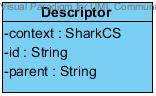
\includegraphics{../Bilder/descriptor.jpg}
		}
		\caption{Konzeption eines Deskriptor}
		\label{fig:descriptor}
	\end{figure}
	
	Dieses Element soll Deskriptor genannt werden. Es besitzt die folgenden
	Parameter:
	
	\begin{itemize}
		\item \textbf{Kontext (context):} Der Kontext ist der Kern des Deskriptor.
		Er bestimmt, welche Kontextpunkte durch ihn aus der Wissensbasis extrahiert
		werden können. Dabei ist es allerdings auch möglich ihm keine Bedeutung 
		zuordnen. Dies ist möglich, wenn der Deskriptor zur	Beschreibung einer
		Beziehung benetzt wird, beispielsweise eines Ordners in einem Dateisystem.
		dabei ist dann nur interessant, welche Kinder dieser besitzt, nicht aber
		die Kontextpunkte, die er beschreibt. So ein Deskriptor soll leerer
		Deskriptor genannt werden.
		\item \textbf{Identifikator (id):} Der Identifikator ist ein Teil des
		Paares, welche die Vater-Kind Beziehung ermöglicht. Des weiteren
		ermöglicht er das wieder auffinden eines bestimmten Deskriptor aus einer
		Liste von Deskriptoren.
		\item \textbf{Vater (parent):} Der Vater ist der andere Teil des Paares,
		welche die Vater-Kind Beziehung ermöglicht. Er erlaubt das Aufwinden des
		Vaters eines Deskriptor. Ebenfalls kann so ein Deskriptor nach seinen
		Kindern	suchen.
	\end{itemize} 	
	
	Man beachte, dass Identifikator und Vater Zeichenketten sind statt, wie
	oft übliche, numerische Werte. Es ist geplant, dass der jeweilige Entwickler
	dafür zuständig ist einen Identifikator zu definieren. Dieser sollte daher
	für Menschen lesbar und interpretierbar sein. Ein Identifikator für einen
	Chat könnte zum Beispiel einfach Chat genannt werden. Oder es könnte sich um
	einen Subject Identifier des Topic Maps Modells sein, dem sich das Shark
	Framework bedient. \\
	
	Hierbei sei angemerkt, dass es sich trotzdem um eine technische Identifikator,
	der von Maschinen und nicht Menschen verwendet wird, handelt. Die Darstellung
	als Zeichenkette dient jegliche als Vereinfachung. Somit ist eine größere
	Auswahl an zu erstellenden Identifikatoren möglich und zeigt Synergien 
	mit dem Topic Maps Modells des Shark Framework auf, da die Subject Identifier
	ein Array von Zeichenketten sind. \\
	
	Des weiteren werden die Väter eines Elements vorerst auf einen Knoten,
	wie in einem einem Baum üblich, beschränkt. Dies kann in diesem Modell später,
	wenn die Notwendigkeit dieser Komplexität besteht, durch das Austauschen des
	parent Parameters durch eine Liste von Zeichenketten auf mehre Väter erweitert
	werden.
	
	\subsubsection{Gleichheit von Deskriptoren}
	
	Mit der Einführung eines Identifikators für Deskriptoren besitzen
	diese nun zwei Definitionen von Gleichheit. Die Unterscheidung soll sein,
	dass ein Deskriptor einem Anderen \emph{gleicht} und ein Deskriptor zu
	einem Anderen \emph{identisch} ist.
	
	\begin{itemize}
		\item \textbf{Ein Deskriptor \emph{gleicht} einem Anderen:} Deskriptor
		sind gleich, wenn ihre Identifikatoren gleich sind. Das heißt, die
		Zeichenketten müssen übereinstimmten.
		\item \textbf{Ein Deskriptor ist \emph{identisch} zu einem Anderen:}
		Deskriptor sind identisch zueinander, wenn alle ihre Elemente glich sind.
		Das heißt, die Zeichenketten des Identifikator und Vater müssen mit denen,
		eines anderen Deskriptor übereinstimmten. Des Weiteren muss der Kontext,
		nach Regeln des Shark Frameworks, identisch sein.
	\end{itemize} 	
	
	Diese Unterscheidung ist notwendig, um das wiederzufinden eines Deskriptor
	sicher zu stellen und doppelte Datenhalten zu verhindern, da der Identifikator
	einen Primärschlüssel darstellt. Anhand dessen kann nach einem bestimmten
	Deskriptor gesucht werde. dennoch muss es möglich sein den Unterschied in
	Vater und Kontext zu erkennen für mögliche Anpassungen. Zum Beispiel könnte
	der Deskriptor von einem anderen Peer geändert worden seien und wurde dann
	versendet, damit sich alle anderen Peers synchronisieren können. In diesem
	Fallbeispiel ist es nötigen, dass der Deskriptor anhand seines Identifikators
	gefunden wird und eine Überprüfung stattfindet, ob dieser angepasst werden
	muss. \\
	
	Geplant ist die Umsetzung für Gleichheit anhand der equals-Methode die ein
	jedes Java-Objekt von Object erbt. Viele Methoden der Collection-API basieren
	darauf, wie beispielsweise die Aussage, ob eine Liste ein bestimmtes Objekt
	einhält. Ob ein Deskriptor zu einem Anderen identisch ist soll anhand einer
	gesonderten Methode implementiert werden.
	
	\subsubsection{Darstellung und Bedeutung von Beziehungen}
	
	In diesem Abschnitt wird genauer auf die Darstellung und Bedeutung von 
	Beziehungen zwischen Datenbereichen eingegangen. Die grundlegende
	Eigenschaften, die einem Deskriptor ermöglichen eine Beziehung darzustellen,
	wurde bereits im vorhergehenden Abschnitt erklärt. Das Grundprinzip ist eine
	Selbstreferenz, die in \autoref{fig:selfref} dargestellt ist.
	
	\begin{figure}[H] 
		\centerline{
			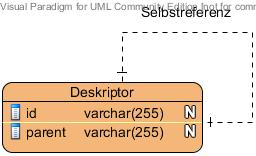
\includegraphics{../Bilder/selfref.jpg}
		}
		\caption{Skizze: Selbstreferenz}
		\label{fig:selfref}
	\end{figure}
	
	Die Abbildung zeigt ein Entity Relationship Diagramm als Skizze. Die 
	Zeichenlimitierung an der Zeichenkette kann hier ignoriert. Der Datentyp 	
	varchar kann verallgemeinert als Zeichenkette interpretiert werden. Die
	Elemente existieren nur in dieser Form aufgrund der Natur des Diagramms.
	Der wichtige Aspekt ist die Selbstreferenz. Über den Fremdschlüssel
	\emph{parent} wird ein Objekt des gleichen Typs referenziert. Dies erlaubt
	uns einen Baum von beliebiger Tiefe zu erstellen. Ein Vater kann auch
	auch beliebig viele Kinder haben, währendes ein Kind nur einen Vater besitzen
	kann.
	
	Folgenden soll die Anwendung dieses Modells die in Abschnitt \ref{sec:social}
	besprochenen Social Media Formaten angewandt werden. Es wird gezeigt, wie es
	konzeptionell angewandt werden kann.
	
	\paragraph{Chat}\mbox{} \\
	
	Die Beziehungen in Chats sind vermutlich am einfachsten zu beschrieben, da
	kaum welche existieren. \autoref{fig:chat_rel} zeigt ein Konzept, wie
	für Beziehungen von Chats.

	\begin{figure}[H]
		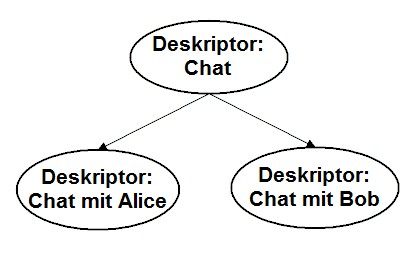
\includegraphics[width=\linewidth]{../Bilder/chat_rel.jpg}
		\caption{Beziehungen von Deskriptoren für Chats}
		\label{fig:chat_rel}
	\end{figure}
	
	Hier existiert genau eine eine Vater-Kind Beziehung. Dabei ist die
	Wurzeln des Baumes nur ein Anker, der andere Deskriptoren zusammenfasst.
	Geht man nach \autoref{fig:chat_rel}, so ist es möglich alle Chats
	zu finden, indem man alle Kinder des Deskriptor Chat findet. Das
	Vaterelement soll hierbei keine Informationen oder Kontextpunkte
	beschrieben. Es dient lediglich der Zuordnung. Der Kontext kann somit als
	leer angesehen werden. Alle Kindelemente des Deskriptor Chat hingeben
	beschreiben genau einen Chat. Die zugehörigen Kontextpunkte sind somit die
	Einträge in dem Chat. Die Beziehung zwischen Deskriptoren wird hier 
	ausschließlich für die Zuordnung zu einer Obergruppe genutzt. 
		
	\paragraph{Forum und Dateisysteme}\mbox{} \\
	
	Forum und Dateisysteme gleichen sich in ihrer Baumartigen Struktur. Sie können
	daher ein ähnliches Modell verwenden. Zum einen gibt es die Einordnung
	in eine Ebene, wie ein Unterforum oder Verzeichnis sein kann. Auf der anderen
	Seite gibt es die Elemente, welche die eigentlichen Daten enthalten. \\
	
	\autoref{fig:forum_rel} zeigt ein Konzept für Beziehungen, welche für die
	Einordnung von Unterforen und Threads in ein Forum darstellt.
	
	\begin{figure}[H]
		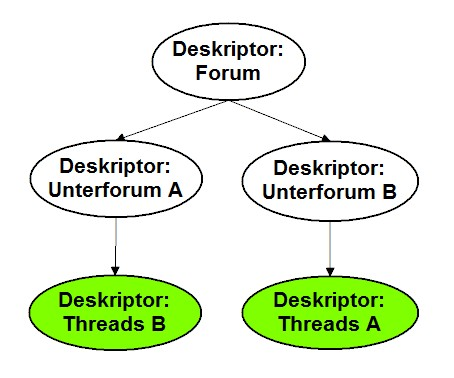
\includegraphics[width=\linewidth]{../Bilder/forum_rel.jpg}
		\caption{Beziehungen von Deskriptoren eines Forum}
		\label{fig:forum_rel}
	\end{figure}
	
	Abgebildet wird die Baumstruktur. Es wird an einer Wurzel begonnen und
	die Beziehungen zeigen auf, welche Unterforen von da an existieren. Die
	Deskriptoren können, wie beim Chat Deskriptor, leer sein und zur zur
	Darstellung der Beziehung verwendet werden. Zumindest ein Blatt muss
	allerdings eine Menge an Kontextpunkten beschreiben. Per Konzept ist ein Thread 
	eine Menge von Kontextpunkten, wobei jeder Punkt genau einem Post entspricht.
	Demzufolge können leere Deskriptoren als reine Unterforen angesehen werden.
	Nicht leere Deskriptoren hingegen schrieben immer einen Thread. Ein nicht
	leerer Deskriptor mit einer Beziehung sollte Aufgrund der Übersichtlichkeit
	nicht verwendet werden. \\
	
	Die Struktur von Dateisystem ist gleich der eines Forum. \autoref{fig:file_rel}
	zeigt die Beziehungen für Verzeichnisse und Dateien.
	
	\begin{figure}[H]
		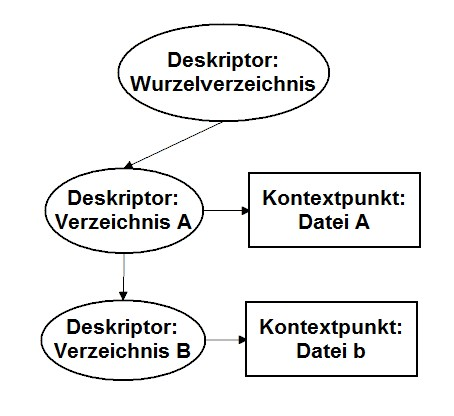
\includegraphics[width=\linewidth]{../Bilder/file_rel.jpg}
		\caption{Beziehungen von Deskriptoren in einem Dateisystem}
		\label{fig:file_rel}
	\end{figure}	
	
	Der konzeptionelle Unterschied zwischen Dateisystem und Forum ist hier, 
	dass ein Kontextpunkt immer genau eine Datei beschreibt, anstatt dass ein
	Thread eine Reihe von Kontextpunkten ist.\\
	
	Man beachte beachte, dass es sich hierbei um ein Konzept handelt.
	Implementieren können anders aussehen. Zum Beispiel ist es möglich und
	eventuell auch sinnvoll, dass eine Datei eine Information an einem Kontextpunkt
	ist. Somit könnte ein Kontextpunkt mehre Dateien enthalten. Das Prinzip des
	Deskriptor ist abstrakt genug um dem Entwickeln hier Freiheit für seine
	Implementieren zu bieten.
	
	\subsubsection{Ein Schema von Beziehungen}
	
	Wie bereist erwähnt gibt es in Java, der Programmiersprache in welcher die 
	zu entwickelnde Softwarekomponente geschrieben werden soll, keine vorgefertigte
	Datenstruktur für Bäume. Von daher muss eine Klasse erstellt werden, welche
	dieses ermöglicht. Im folgenden ist beschrieben, welche Aufgaben sie erfüllen
	soll.
	
	\newpage
	\begin{itemize}
		\item \textbf{Speichern und laden der Deskriptoren:} Das Schema soll die
		 Deskriptoren an der Wissensbasis speichern und aus dieser laden können.
		 Dies soll sowohl für alle gehen als auch für einen bestimmten
		 Identifikator.
		\item \textbf{Vater-Kind Beziehung:} Das Schema stellt die eigentlichen
		Vater-Kind Beziehungen da. Daher ermöglicht es einem Deskriptor Kinder
		hinzuzufügen, sowie einen Vater zu setzen. Wird ein neuer Vater gesetzt,
		so wird der alte überschrieben. Auch muss sichergestellt werden, dass
		es zu keiner Schleife bei den Bezeichnungen kommt, damit immer ein Baum
		mit einer Wurzel und Blättern existiert.
	\end{itemize}
	
	\subsubsection{Extraktion von Daten}
	\label{sec:extraction}
	
	Deskriptoren existieren um Datenbereiche zu beschrieben. Als solches ist es
	muss de Möglichkeit bestehen Kontextpunkte anhand des Kontext eines Deskriptor
	zu extrahieren. Dabei sollen die folgenden Möglichkeiten bestehen:
	
	\begin{itemize}
		\item \textbf{Extraktion des Kontext des Deskriptor:} Nur die Kontextpunkte
		zum Kontext des aktuellen Deskriptor werden extrahiert.
		\item \textbf{Extraktion des Unterbaumes:} Die Kontextpunkte des aktuellen
		 Deskriptor, sowie alle Kontextpunkte seiner Kinder werden extrahiert
		\item \textbf{Extraktion des gesamten Baumes:} Die gesamten Kontextpunkte
		des Baumes werden extrahiert. Das heißt, es wird zuerst die Wurzel des
		Baumes gesucht und dann der Unterbaum, inklusive der Wurzel selbst,
		extrahiert.
	\end{itemize}
	
	\subsection{Synchronisation}
	
	In diesem Abschnitt wird der Algorithmus zur Synchronisation der Daten
	konzipiert. Dazu wird der Algorithmus der SyncKB von des Shark Framework 
	mit dem im letzten Abschnitt beschrieben Deskriptor erweitert.
	
	\subsubsection{Mängel der aktuellen SyncKB}
	
	Bevor ein Algorithmus entworfen wird sollen die Mängel der aktuellen 
	Synchronisation besprochen werden. \autoref{fig:sync_now} zeigt nochmal eine
	Skizze des Algorithmus des SyncKP aus Abschnitt \ref{sec:SyncKB}. Für den
	eine Erklärung des sequenziellen Ablauf siehe \autoref{fig:SyncSeq} und
	Nachfolgende Beschreibung.
	
	\begin{figure}[H]
		\centerline{
			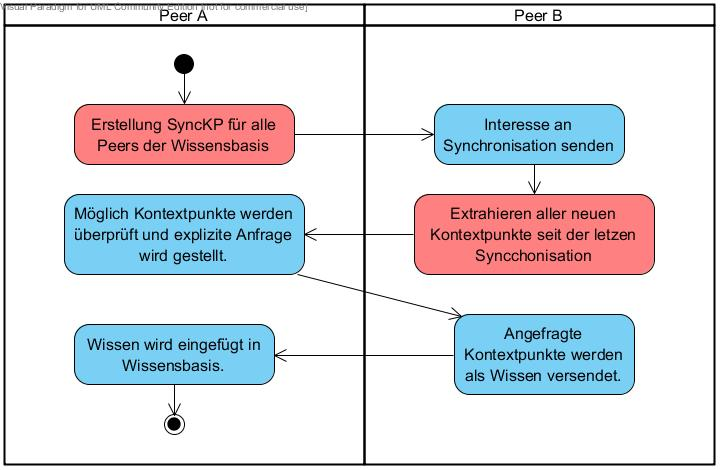
\includegraphics[scale=0.495]{../Bilder/sync_flaws.jpg}
		}
		\caption{Skizze: Synchronisation Algorithmus der aktuellen SyncKB}
		\label{fig:sync_now}
	\end{figure}
	
	In der aktuellen Form zeigt der Algorithmus der SyncKB zwei gravierende Mängel
	auf.
	
	\begin{enumerate}
		\item \textbf{Synchronisation mit allen Peers:} Der Algorithmus nimmt alle
		Peers der Wissensbasis daher und synchronisiert mit diesen. Für die
		Fallbeispiele dieser Arbeit soll aber nur mit bestimmten Peers eine
		Synchronisation stattfinden. So wären dies Beipeilweise in einem Chat die
		Teilnehmer. In einem Forum alle Mitglieder dieses. Diese Menge ist
		nicht zwangsweise gleich mit allen Peers in der Wissensbasis.
		\item \textbf{Synchronisation aller Kontextpunkte:} Ebenfalls
		synchronisiert der Algorithmus alle Kontextpunkte einer Wissensbasis. 
		dem Namen dieser Arbeit Name ist allerdings eine partiellen Synchronisation
		erwünscht.		
	\end{enumerate}
	
	\subsubsection{Abstraktion von der SyncKB}
	
	Aufgrund der im letzten Abschnitt beschrieben Mängel soll eine Abstraktion der
	SyncKB vorgenommen werden. Genauer soll die Klasse SyncKP abstrahiert werden.
	Wenn hier von einer Abstraktion gesprochen wird	ist hier von einer Abstraktion 
	in der objektorientierte Programmierung die Rede. Die Klasse SyncKP soll in
	eine abstrakte Klasse AbstractSyncKP umgewandelt werden. Der Entwickler, der
	von dieser erbt ist dann, ist dann verpflichtet die abstrakten Methoden dieser
	Klasse zu implementieren. Ziel dieser ist das erreichen	folgender Aktionen:
	
	\begin{itemize}
		\item \textbf{Entscheidung ob ein Interesse besteht:} Es sollte im 
		Ermessen des Entwicklers liegen, ob eine Interesse zur Synchronisation
		für eine Knowledge Port interessant ist oder nicht. Je nach Fall kann
		es vorkommen, dass bestimmte Dimensionen des gesendeten Interesse überprüft
		werden müssen oder nicht. Dem Entwickler soll hier Freiheit geben werden
		dies selbst zu entscheiden.
		\item \textbf{Finden des Identifikator:} Die bestehende Implementation der
		SyncKB benötigt einen Identifikator woran es seine Metadaten speichern
		kann. Dieser Identifikator ist nicht gleich mit dem Identifikator eines
		Deskriptor. Es handelt sich um ein tatsächliches Tag an dem Properties
		gespeichert werden können. Im künstlichen Interesse der aktuellen SyncKB
		ist dies eine Tag in der Topic Dimension, dass schlicht dem halten von
		Metadaten dient.
		\item \textbf{Zusammenstellen des Angebotes:} Wie in Abschnitt
		\ref{sec:extraction} erläutert gibt es mehre Möglichkeiten Wissen
		anhand eines Deskriptor zu extrahieren. Daher ist es sinnvoll dem
		Entwickler zu überlassen wie genau das Wissen aus der Wissensbasis zu
		extrahieren ist. 
	\end{itemize} 	
	
	\newpage
	\section{Implementierung}
	
	In diesem Kapitel wird die Implementierung besprochen. Es wird gezeigt, wie
	das Konzept in Java Quellcode implementiert wurde und welche Techniken dazu
	verwendet wurden. Des Weiteren wird besprochen, wie entworfenen Klassen 
	genutzt werden können.
	
	\subsection{Deskriptor und Schema}
	
	Deskriptor und Schema werden in die zwei Klassen ContextSpaceDescriptor
	und DescriptorSchema aufgeteilt. Die Klasse ContextSpaceDescriptor ist dabei
	eine reine Beschreibung eines Datenbereiches. Die Klasse DescriptorSchema
	organisiert die Deskriptoren in einer Baumstruktur und ermöglicht das
	Speichern und Laden dieser von einer Wissensbasis. \autoref{fig:impl_schema}
	zeigt das Klassendiagramm beider.
	
	\begin{figure}[H]
		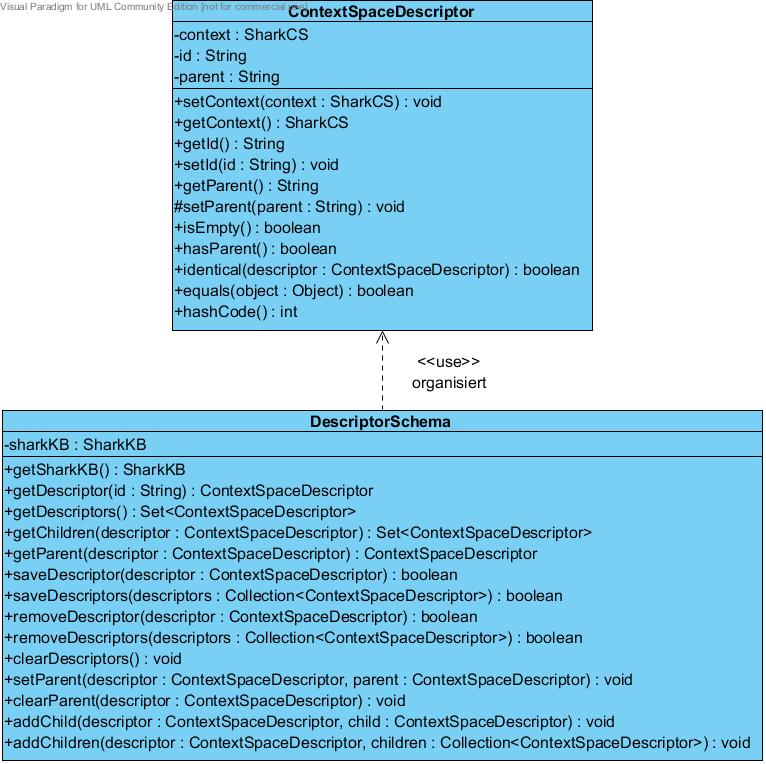
\includegraphics[width=\linewidth]{../Bilder/impl_schema.jpg}
		\caption{Klassendiagramm: Deskriptor und Schema}
		\label{fig:impl_schema}
	\end{figure}	
	
	Konstruktoren und private Methoden wurden hier vernachlässigt. Eine
	explizite Beschreibung aller Klassen kann der Javadoc Dokumentation gefunden
	werden (siehe \autoref{sec:CD}). \\
	
	Im folgenden soll auf die Verwendung dieser Klassen eingegangen werden.
		
	\paragraph{Deskriptor}\mbox{} \\
	
	Die Klasse ContextSpaceDescriptor hat die aus Abschnitt \ref{sec:desk} 
	beschrieben drei Parameter Kontext(context), Vater(parent) und
	Identifikator(id). Für dieses Methoden gibt es jeweils Setter und Getter
	Methoden. Zu beachten dabei ist, dass der Setter für den Vater auf die
	Sichtbarkeit protected gesetzt ist. Der Entwickler soll die	Vater-Kind
	Beziehungen über das Schema konfigurieren, welche Fehlerprüfungen durchführt,
	nicht über die Klasse ContextSpaceDescriptor selbst. Das der Getter für
	parent die Sichtbarkeit public besitzt dient nur zu Debugging und Logging
	Zwecken.\\
	
	Des Weiteren gibt es eine Reihe von Methoden, welche folgende Eigenschaften
	prüfen:
	
	\begin{itemize}
		\item \textbf{Leere:} Die isEmpty Methode prüft ob ein Deskriptor
		leer ist. Ein Deskriptor ist leer, wenn der Parameter context null ist.
		\item \textbf{Zwei Deskriptoren sind gleich:} Die von Object überschieben
		equals Methode pürft ob zwei Deskriptoren gleich sind. Ein Deskriptor
		gleicht einem anderen, wenn die Parameter id gleich sind. Mit dieser
		Prüfung	auf Gleichheit werden Features des Collection Framesworks genutzt
		von Java genutzt. Die contains Methode zum Beispiel gibt so wieder ob
		in einer Collection bereits ein Deskriptor mit dem gleichen Identifikator
		existiert. Zusätzlich ist auch die hashSet Methode überschrieben. Das
		ausschlaggebende Element ist auch hier der Parameter id. Demzufolge
		ist auch der Hash zweier Deskriptoren gleich, wenn ihr Identifikator 
		gleich ist.
		\item \textbf{Zwei Deskriptoren sind identisch:} Die identical Methode
		prüft ob ein Deskriptor identisch zu eine anderen Deskriptor ist. Dies
		ist der Fall, wenn Die Parameter id und parent die Gleicheit aufweisen,
		sowie die context Parameter identisch sind nach den Regeln des Shark
		Frameworks. Somit können Deskriptoren auf Untershcide in überprüft werden,
		obwohl sie den gleiche Identifikator besitzen.
	\end{itemize}
	
	\paragraph{Schema}\mbox{} \\
	
	Die Klasse DescriptorSchema ermöglicht sowohl das Speichern, wie auch das
	Laden von Deskriptoren aus der Wissensbasis als auch der konfigurieren von
	Beziehungen	zwischen Deskriptoren. Nach außen ist sie die Klasse, welche
	die Beziehungen enthält, auch wenn die Schlüssel intern an der Klasse
	ContextSpaceDescriptor beschrieben sind. Sie kann ähnlich einem 
	Datenbankmanagementsystem gesehen werden. \\
	
	Ein Schema basiert immer auf einen Wissensbasis, aus der die Daten geladen und
	gespeichert werden. Des weiteren besitzt sie folgende Features:
	
	\begin{itemize}
		\item \textbf{Speichern und Laden von Deskriptoren:} Deskriptoren können
		an der Wissensbasis, die das Schema verwendet, gespeichert werden und.
		geladen werden. Hierzu einhält die Klasse die Methoden getDescriptor,
		getDescriptors, saveDescriptor, saveDescriptors, removeDescriptor und
		saveDescriptors. Das löschen des gesamten Schemas ist mittels 
		clearDescriptors möglich. Deskriptoren werden immer in einem Set gehalten,
		das heißt alle Elemente der Liste sind unterschiedlich. Unterschiedlich
		bezieht sich hierbei die Gleichheit, das heißt sie besitzen alle
		unterschiedliche Identifikatoren. Das Speichern eines Deskriptor mit dem
		gleichen Identifikator wie ein bereits existierender Deskriptor
		überschriebt kommt einem Überschrieben gleich.
		\item \textbf{Konfigurieren von Vater-Kind Beziehungen:} Über die Methoden 
		addChild, addChildren, setParent können Vater-Kind Beziehungen aufgebaut
		werden. Zu beachten ist, dass ein Deskriptor immer nur einen Vater
		haben kann. Wird ein neue gesetzt, so wird der Alte überschrieben. Das
		hinzufügen eines Kindes zu einem Deskriptor ist gleich dem Setzen eines 
		Vaters (Parameter: descriptor) für den Parameter child. Existiert ein
		Deskriptor nicht im Schema oder würde das Hinzufügen zu einer
		Schleife führen, also die Baumstatur verletzen, so erzeugt dies einen
		Fehler.	Ein Vater kann über die clearParent Methode gelöscht werden. Über
		die getChildren	und getParent können Vater und Kinder eines Deskriptor
		erhalten werden.
	\end{itemize}
	
	\subsection{Serialisierung des Schemas}
	
	Wie in Abschnitt \ref{sec:konz_serialisierung} erklärt soll XML unter
	Zuhilfenahme das im Java Development Kit enthalten JAXB zum Serialisieren
	des Schemas verwendet werden. Hierzu sind die Klasse ContextSpaceDescriptor
	über entspreche	Annotations ausgestattet. Für den Parameter context wurde
	eine entsprechender XmlAdapter (siehe \cite{XmlAdapter}) geschrieben, der
	die Serialisierung einer SharkCS Klasse unter Zuhilfenahme der im Shark
	Framework existierenden Klasse XMLSerializer für JAXB ermöglicht. \\
	
	Aufgrund der Annotations wurde auch drauf verzichtet ein Interface zur Klasse
	ContextSpaceDescriptor zu erstellen oder sie abstrakt zu gestalten. Sie wurde
	als normales Java Objekt entworfen das einfach wie eine Java-Bean genutzt
	werden kann. \\
	
	In in der JAXB 2.2 Specification, Section 4.2 JAXB Context \cite{JAXB} steht
	folgendes beschrieben: 
	
	\emph{
		\begin{quote} 
			"To avoid the overhead involved in creating a JAXBContext instance,
			a JAXB application is encouraged to reuse a JAXBContext instance."
		\end{quote}
	}
	
	Aus diesem Grund wurde das Factory Pattern für die Erstellung eines JAXBContext
	benutzt. \autoref{fig:factory} skizziert dieses.
	
	\begin{figure}[H]
		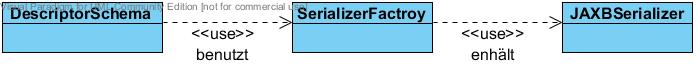
\includegraphics[width=\linewidth]{../Bilder/factory.jpg}
		\caption{Skizze: Factroy Pattern für JAXB Serialisierung}
		\label{fig:factory}
	\end{figure}	
	
	Der JAXBContext ist in der Klasse JAXBSerializer enthalten. Für jede Instanz
	dieser Klasse wird ein einer JAXBContext angelegt. Um dies zu verhindern wird
	die Factory Klasse SerializerFactroy benutzt. Diese folgt dem Singleton Pattern
	und enhält genau einen JAXBSerializer der für Deskriptoren konfiguriert ist. 
	Das Schema kann an diesen über eine Methode abrufen. Sollten weitere Klassen
	einen einen JAXBSerializer für Deskriptoren benötigen, so kann die Instanz 
	über SerializerFactroy wiederverwendet werden. Somit wird auch der JAXBContext
	wiederverwendet und Overhead vermeiden.
	
	\newpage
	\section{Tests}
	
	\newpage
	\section{Fazit}
	
	
	\newpage
	\section{Quellenverzeichnis}	
	
	\printbibliography[type=article,heading=subbibliography,title={Artikel}]
	\printbibliography[type=book,heading=subbibliography,title={Bücher}]
	\printbibliography[type=manual,heading=subbibliography,title={Handbücher}]
	\printbibliography[type=misc,heading=subbibliography,title={Publikationen}] 			\printbibliography[type=report,heading=subbibliography,title={Spezifikationen}]
	\printbibliography[type=online,heading=subbibliography,title={Webseiten}]

	\newpage
	\section{Abbildungsverzeichnis}
	\makeatletter
		\@starttoc{lof}% Print List of Figures
	\makeatother
		
	\newpage	
	\begin{appendix}
	
	\section{CD-ROM zur Arbeit}
	\label{sec:CD}
	
	Die beiliegende CD-ROM zur Arbeit enthält die folgenden Inhalte.
	
	\begin{itemize}
		\item \textbf{Masterarbeit.pdf:} Diese Arbeit im PDF Format.
		\item \textbf{Verzeichnis Quellcode:} Der Quellcode zu dieser Arbeit
		als ein Maven-Projekt. Das Projekt bringt alle Abhängigkeiten mit
		und kann über den \emph{install} Befehl von Maven gebaut werden. \\
		Weitere Informationen zu maven sind unter \url{https://maven.apache.org/}
		zu finden.
		\item \textbf{Dokumentation:} JavaDoc Dokumentation des Quellcodes, sowie
		ein Cobertura und PMD Report zur Qualitätssicherung. 
	\end{itemize} 
	
	Die Quellen existieren zusätzlich in GitHub unter 
	\url{https://github.com/SharedKnowledge/Incubator/tree/master/Descriptor}. \\
	
	Das Maven Projekt ist konfiguriert eine Cobertura Report über den Maven Befehl 
	\emph{cobertura:cobertura} zu erstellen. Ein PMD Report kann über den Maven
	Befehl \emph{pmd:pmd} erstellt werden.
	

	\newpage	
  	\section{Eigenständigkeitserklärung}
  	Hiermit versichere ich, dass ich die vorliegende Masterarbeit selbstständig und
  	nur unter Verwendung der angegebenen Quellen und Hilfsmittel verfasst habe. Die
  	Arbeit wurde bisher in gleicher oder ähnlicher Form keiner anderen
  	Prüfungsbehörde vorgelegt. \\ \\
  	
 	Datum: \hspace{10pt} Berlin, 12. Oktober 2015 \hspace{30pt} Unterschrift:

	\end{appendix}
  	
\end{document}